\section{Abstract Correlating Semantics}\seclabel{AbstractSem}

In this section, we introduce our correlating abstract domain which allows bounded representation of product program state while focusing on maintaining equivalence between correlated variables. This comes at the cost of an acceptable lose of precision of other state information. We represent variable information using standard relational abstract domain. As our analysis is path sensitive, we allow for a set of abstract sub-states, each adhering to a certain path in the product program. To assure we only allow correct paths, that truly abstracts our collecting semantics of correlated executions, our abstraction will initially assume equality on all inputs. This power-set domain records precise state information but does not scale due to exponential blow-up of number of paths. We describe minimization techniques, or canonization, that reduce the super-state size by joining part of its sub-states together (using the sub-domain lossy join operation). We select these sub-states according to criteria that allows separation of equivalence preserving paths thus achieving better precision. We start off by abstracting the collecting semantics in \subref{ConcreteCorrelatingSemantics}.

In the following, we assume an abstract relational domain $RD = \langle RC, \sqsubseteq_{RD} \rangle$ equipped with operations $\sqcap_{RD}$, $\sqcup_{RD}$ and $\nabla_{RD}$, where $RC$ is a set of relational constraints over the variables in $Var$, and do not go into further details about the particular abstract domain as it is a parameter of the analysis. We also assume that the sub-domain $RD$ allows for a sound over-approximation of the concrete collecting semantics (given a sound interpretation of program operations).

\paragraph{Correlating Abstract State} \deflabel{CorrelatingAbstractState}
A correlating abstract program state $\C{\sigma_{\times}}$, is a tuple $\langle l_{\times}, S^{RD} \rangle \in \C{\Sigma}$, where $l_{\times}$ is a label in the product program and $S_{RD}$ is a set of abstracts from the sub-domain $RD$, such that each $rd \in S_{RD}$ will abstract a certain \textbf{path} in the product program. We achieve that by instrumenting each $\sigma_{\times} = last(pre(\pi_{\times}))$ in the collecting semantics $CS(l_{\times})$ with the sequence of branches taken up to $\sigma_{\times}$ in $pre(\pi_{\times})$. This is easily achieved by using \emph{guard} values as they are recorded along the trace and we denote $path(\sigma_{\times})$ as the sequence of branches $b_0,...,b_n$ i.e. guard values ($b_i = <g,{T/F}>$), that led up to $\sigma_{\times}$. Therefore we define for every path $p_i$ in the product program the group of concrete correlating states that exist at the end of that path denoted $\Sigma_{\times}^{p_i} \triangleq \{ \sigma_{\times} | path(\sigma_{\times}) = p_i \}$. Finally we define the abstract state itself as $\C{\sigma_{\times}} \triangleq { rd | rd = ABS_{RD}(\Sigma_{\times}^{p_i}) \wedge p_i is a path in P \times P)}$. For example, the abstraction of \figref{MatchingProblemExamplePrograms}'s product program collecting semantics at labels $(lab,lab')$ will first collect together all trace prefixes that iterate the loop 0 times: $\Sigma_{\times}^{p_0} = \{  (x=0,i=0,x'=0,i'=0), (x=1,i=0,x'=1,i'=0), (x=2,i=0,x'=2,i'=0), ... \}$ and abstract them using the relational sub-domain to get $rd_{0} = \{x=x',i=i'=0\}$ which correctly expresses the fact that equivalence is kept in case none of the loops iterate. The next path to be abstracted would be where both loops iterate once i.e. $p_1 = <g,F>,<g',F>$ which also maintains equivalence and will be abstracted as $rd_{1} = \{x=x',i=i'=1, x \geq 1\}$. The next path however, which iterates the $P'$ loop twice but only once for the $P$ loop, $p_2 = <g,F>,<g',F>,<g,T>,<g',F>$ will not maintain equivalence as it will abstract $\Sigma_{\times}^{p_2} = \{  (x=1,i=1,x'=1,i'=2), (x=2,i=2,x'=2,i'=2), (x=3,i=2,x'=3,i'=2), ... \}$ as $rd_{2} = \{x=x',2 \leq i \geq 1, i'=2\}$. We mention that the abstract $rd$ ignores the separation of concrete states of $P$ and $P'$ and abstracts both variable data together. In fact, the ability to maintain direct relationships between the two sets of variables (and specifically those matched by $VC$) is crucial for maintaining equivalence.
 
Every path in the product program will be represented by a single abstract of the sub-domain. As a result, all \textbf{traces prefixes} that follow the same path to $l_{\times}$ will be abstracted into a single sub-state of the underlying domain. This abstraction fits semantics differencing well, as inputs that follow the same path display the same behavior and will usually either keep or break equivalence together, allowing us to separate them from other behaviors (it is possible for a path to display both behaviors as in \figref{PathProblemExamplePrograms} and we will discuss how we are able to manipulate the abstract state computed at the end to separate equivalent behaviors from the ones that offend equivalence). Another issue to be addressed is that fact that our state is again potentially unbound as there may be an infinite number of paths in the program (due to loops).

\paragraph{Computing Abstract State with Our Analysis} \deflabel{ComputingAbstractState}
We compute the correlating abstract state at each label $\C{\sigma_{\times}}$ by using means of abstract interpretation and program analysis. We interpret our correlating program (described in \secref{CorrelatingProgram}) which is a semantic preserving reduction over the much more arbitrary product program, using a standard fixed-point analysis algorithm, and apply interpreted operations on the set of sub-states of the current state $S_{RD}$. Our initial state explicitly assumes equality on all input variables (by adding a $v=v'$ constraint for every input variable $v$ where $v'=VC(v)$) to allow for sound checking of equivalence. This also allows for pruning of unfeasible paths where inputs diverge\COMMENT{ (though we may still interpret some as feasible due to incompleteness of program operations representation, for example bitwise operations)}. To adhere to the representation of traces in the abstract state, our join operation is in fact set union, thus indeed every prefix that reaches a certain program label will be awarded its own $rd$. Let us explicitly define the operations of the domain in our analysis:
\begin{itemize}
\item $S^{RD}_1 \sqsubseteq S^{RD}_2 \Longleftrightarrow \forall rd_1 \in G_1 \exists rd_2 \in G_2 : rd_1 \sqsubseteq_{RD} rd_2$
\item $S^{RD}_1 \sqcap S^{RD}_2 \equiv { rd_1 \sqcap_{RD} rc_2 | rd_1 \in G_1 \wedge rd_2 \in G_2}$
\item $S^{RD}_1 \sqcup S^{RD}_2 \equiv S^{RD}_1 \cup S^{RD}_2$
\end{itemize}
Next we define two more operations: Canonization (denoted $\odot$) - which allows for minimization of state size according to equivalence criteria and Widening (denoted $\nabla$) - which allows reaching a fixed-point when handling loops.

\COMMENT{One advantage of our correlating domain over using two separate domains, is the ability to preserve equivalence in the face of non-linear operations - this argument may be too thin to include.}

\begin{figure}
%\lstset{numbers=left, language=C, basicstyle=\ttfamily\scriptsize,emph={},emphstyle=\textbf,escapechar=\%}
\begin{tabular}{cc}
\centering
\begin{lstlisting}
int f(int x) {
    return x;
}
\end{lstlisting}
&
\begin{lstlisting}
int f'(int x) {
    return 2*x;
}
\end{lstlisting}
\end{tabular}
\figlabel{PathProblemExamplePrograms}
caption{single path differentiation candidates}
\end{figure}

\paragraph{Canonization}
We can see from our motivating example that it is not feasible to allow our correlating domain to keep diverging and double in size with every conditional as it will exponentially blow up the analysis run-time and memory. Instead, we employ an equivalence conserving canonization technique such that at every canonization point we will partition the sub-states according to the set of variables to which they hold equivalence for and join these all together into one abstract, using the sub-domain lossy join. This bounds the number of abstracts in the state to $2^{|V|}$ for variables correlated $VC$. This fine grained equivalence checking is successful in telling apart paths that hold equality for none, some or all of the variables. For instance in \figref{MatchingProblemExamplePrograms}, our canonization will tell apart the sub-state that hold equivalence for all variables $\{i=i'=x=x'=0\}$ from the rest that hold equivalence for $x$ alone and join them all together into the $\{x=x',i \leq x, i' \leq 2x'\}$ state. The fact that we did not lose equivalence altogether is beneficial as we are able to report that the input variable $x$ did not diverge which may be of use in case \scode{foo} had used $x$ further down the road.

\paragraph{Widening}



\subsection{Correlating Abstract State Differencing} \sublabel{CorrelatingAbstractDiff}
Given a state in our correlating domain, we want to determine whether equivalence is kept and if so under which conditions it is kept (for partial equivalence) or determine there is difference and characterize, as much as possible, this difference. As our state may hold several sub-states, each holding different equivalence data, we can provide a much more verbose answer regarding whether equivalence holds. We partition our sub-states according to the set of variables they hold equivalence for and report the state for each equivalence partition class. Since we instrument our correlating program to preserve initial input values, for some of these states we will also be able to report input constraints thus informing the user of the input ranges that maintain equivalence. In the cases where equivalence could not be proved, we report the offending states and apply a differencing algorithm for extraction of the delta. \figref{PathProblemExamplePrograms} shows an example of where our analysis is unable to prove equivalence (as it is sound), although part of the state does maintain equivalence (specifically for $x=0$). This is due to the abstraction being to coarse. We describe an algorithm that given a sub-state $rd \in RD$, computes the differentiating part of the sub-state (where correlated variables disagree on values) by splitting it into parts according to equivalence. This is done by treating the relational constraints in our domain as geometrical objects and formulating delta based on that.

\paragraph{Correlating Abstract State Delta} \deflabel{CorrelatingAbstractStateDelta}
Given a sub-state $rd$ and a correspondence $VC$, the correlating state delta $\triangle_{A}(rd)$, computes abstract state differentiation over $rd$. The result is an abstract state $\sqsubseteq rd$ approximating all concrete values for variables correlated by $VC$, that differ between $P$ and $P'$. Formally, the delta is simply the abstraction of the collecting semantics deltas $\alpha(\triangle_{CS}^{+}), \alpha(\triangle_{CS}^{-})$ i.e. an abstraction of the set differencing operation. But it is not clear as to how we compute this set differencing on the correlating abstraction. Instead, we consider the geometric representation of the domain and applied operations there for the extraction of delta, as following:
\begin{enumerate}
\item $rd_{\equiv}$ is a state abstracting the concrete states shared by the original and patched program. It is achieved by computing: $rd_{\equiv} \triangleq rd|_{V=V'} \equiv rd \sqcap \bigwedge\{ v = v' | VC(v) = v'\}$.
\item $\overline{rd_{\equiv}}$ is the negated state i.e. $RD \setminus rd_{\equiv}$ and it is computed by negating $rd_{\equiv}$ (as mentioned before, all logical operations, including negation, are defined on our representation of an abstract state).
\item Eventually: $\triangle_{A}(rd) \triangleq rd \sqcap \overline{rd_{\equiv}}$ abstracts all states in $P \times P'$ that where correlated variables values do not match.
\item $\triangle_{A}(rd)^{+} = \triangle_{A}(rd)|_{V'}$ is a projection of the differentiation to display values of $P'$ alone i.e. "added values".
\item $\triangle_{A}(rd)^{-} = \triangle_{A}(rd)|_{V}$ is a projection of the differentiation to display values of $P$ alone i.e. "removed values".
\end{enumerate}
Applying the algorithm on \figref{PathProblemExamplePrograms}'s $P$ and $P'$ where $rd = \{ retVal' = 2retVal \}$ will result in the following: 
\begin{enumerate}
\item $rd_{\equiv} = \{ retVal' = 0, retVal = 0 \}$.
\item $\overline{rd_{\equiv}} = [ \{ retVal' > 0 \}, \{ retVal' < 0 \}, \{ retVal > 0 \}, \{ retVal < 0 \} ]$
\item $\triangle_{A}(rd)  = [ \{ retVal' = 2retval, retVal' > 0 \}, \{ retVal' = 2retval, retVal' < 0 \}, \{ retVal' = 2retval, retVal > 0 \}, \{ retVal' = 2retval, retVal < 0 \} ]$
\item $\triangle_{A}(rd)^{+} = [ \{ retVal' > 0 \}, \{ retVal' < 0 \} ]$
\item $\triangle_{A}(rd)^{-} = [\{ retVal > 0 \}, \{ retVal < 0 \}]$
\end{enumerate}
We see that displaying the result in the form of projections is ill-advised as in some states differentiation data is represented by relationships on correlated variables alone, thus projecting will lose all data and we will be left with a less informative result. A geometrical representation of $\triangle_{A}$ calculation can be seen in \figref{Delta}.

\begin{figure}
\imagetop{
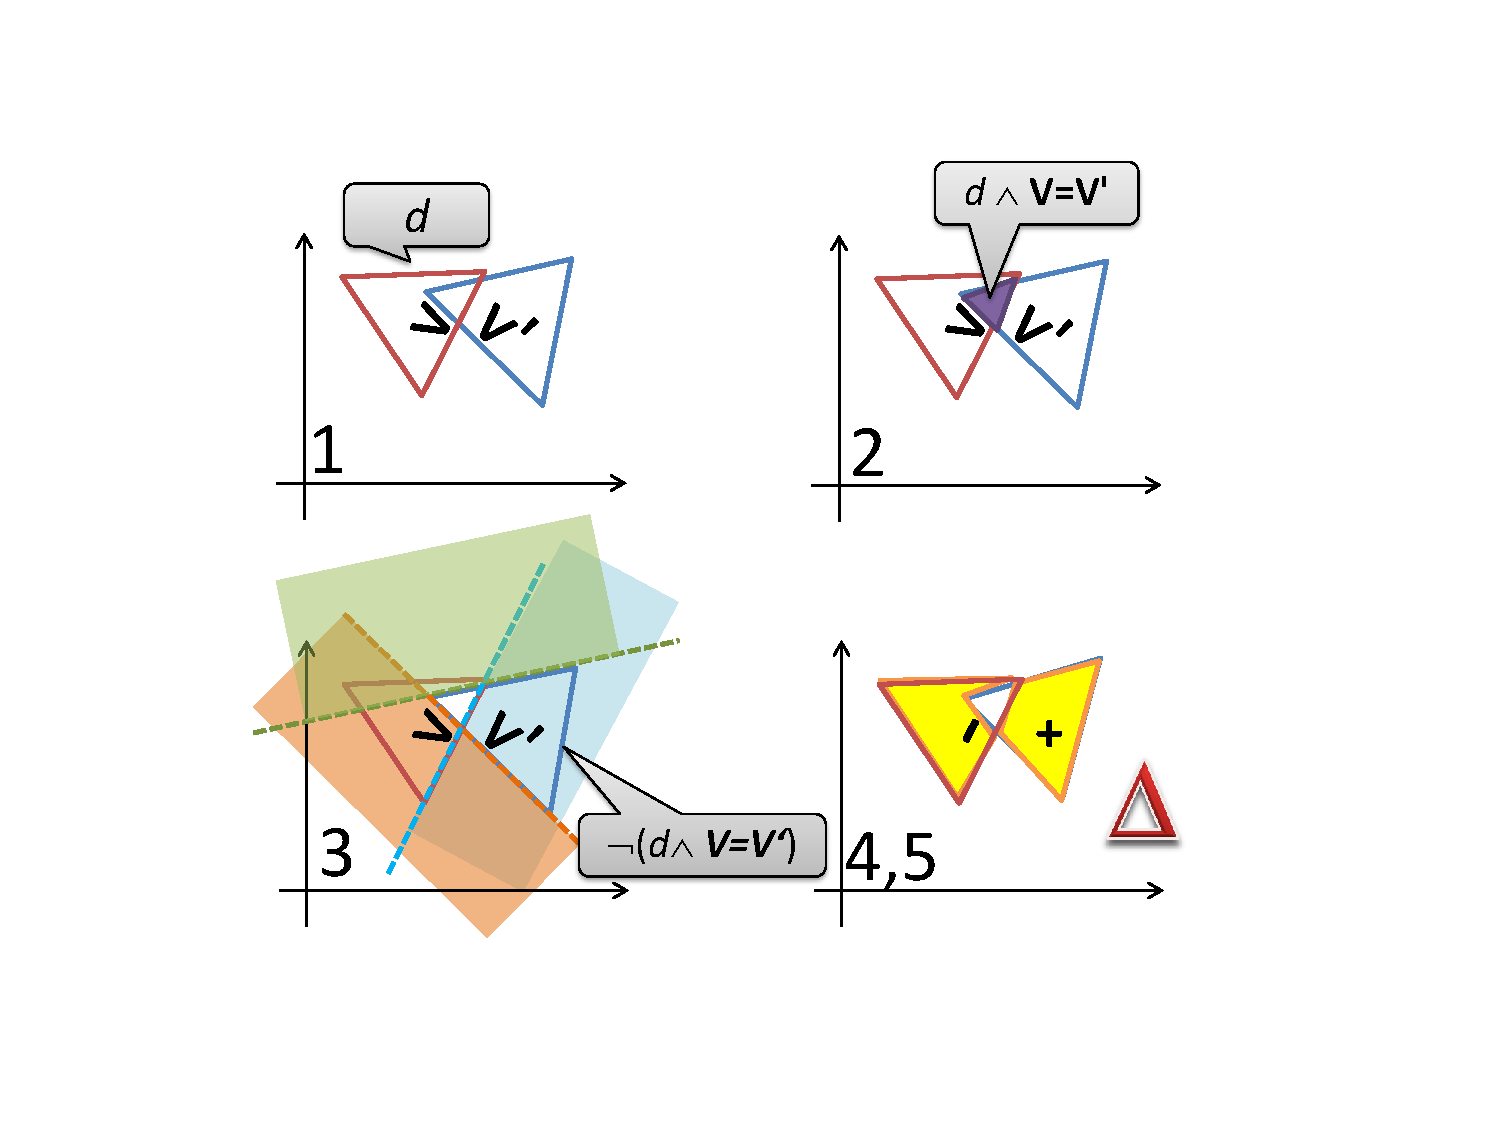
\includegraphics[width=3.0in,clip=true,trim = 100pt 100pt 300pt 300pt]{figures/delta}
}
\caption{Delta computation geometrical representation.}\figlabel{Delta}
\end{figure}

\begin{algorithm}
\small
\DontPrintSemicolon
%\linesnumbered
\SetAlgoLined
\SetAlgoSkip{bigskip}
\KwIn{Abstract state $rd$}
\KwOut{Abstract difference - $\triangle(rd)$}
$rd_{\equiv} \leftarrow rd \sqcap \bigwedge\{ v = v' | VC(v) = v'\}$\;
$\overline{rd_{\equiv}} \leftarrow \neg rd_{\equiv} = \{ \neg c | c \in rd_{\equiv}\}$\;
Foreach $rd_i \in \overline{rd_{\equiv}}$:
    $\triangle(rd) \leftarrow \triangle(rd) \cup (rd \sqcap rd_i$)\;
\Return $\triangle(rd)$
\caption{Compute Abstract Difference.}\label{Alg:AbsDiff}
\end{algorithm}
%% RESET THE ALGORITHMS COUNTER TO PUSHBACK INC FROM FUNCTIONS
\setcounter{algocf}{1}


From this point forward any mention of 'delta' (denoted $\triangle$) will refer to the correlating abstract state delta (denoted $\triangle_{A})$. We claim that $\triangle$ is a correct abstraction for the concrete state delta which allows for a scalable representation of difference we aim to capture.
